\subsection{Set Cover Problem}
Input: Universe of elements $U = \{1, \cdots, n\}$. A collection of subsets of $U$, $\mathfrak{S} = \{S_1, S_2, \cdots, S_m\}$, where each $S_i \subset U$. 

Set cover decision problem: 
\begin{itemize}
	\item Instance: $U$, $\mathfrak{S}$ and given a number $k$.
	\item Question: is there a sub-collection $\mathfrak{f}' = \{S_{i1}, S_{i2}, \cdots, S_{ik}\}$ (at most $k$ sets), such that $\cup_{j=1}^k S_{ij} = U$.
\end{itemize}

Set Cover is in a NP problem. The certificate for a YES-instance is just the sub-collection $\mathfrak{f}'$. It is easy to check whether the sub-collection covers all the elements in the universe and has at most $k$ sets.

Set cover is actually a NP hard problem since it is a generalization of vertex cover problem.


We can show VC reduces to SC in polynomial time. VC $\preccurlyeq_P$ SC. In general, reduce a particular case to a general case would be easy, which is the case in our problem.

Given instance $\langle G, k \rangle$ of VC, we create an instance of set cover as follows:
Let the universe be the set of edges in $G$. $U = \{e_1, e_2, \cdots, e_n\}$. For each vertex $v \in G$, create a subset $S_V = \{e \in E: e \text{ has $v$ as one of its end points.}\}$. Use the same $k$ as the number of vertex sets as the number of sets in SC.
\begin{figure}[H]
	\centering
	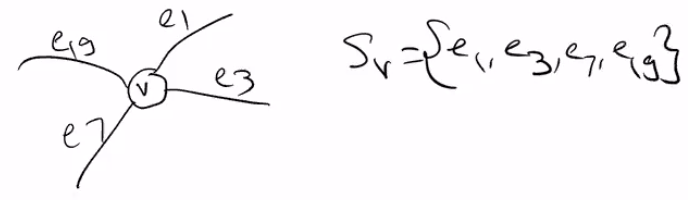
\includegraphics[width=0.5\textwidth]{fig/vs-reduce-to-sc.png}
\end{figure}

If the starting instance is a YES instance of VC, then the reduction produce YES-instance of SC. Conversely, if the instance of SC we produce is a YES instance, then the starting instance must be a YES instance of vertex cover.

\subsection{Set Cover Optimization}

\subsubsection{Greedy Algorithm}
Set Cover Optimization is NP-hard. Approximation algorithm for set cover using a greedy strategy. Recall that the goal is to cover all the vertices. So naturally the first choice of greedy algorithm would be the set that cover as much vertices as possible.

Algorithm $G$:
$R$ is the set of uncovered elements. $C$ is a collection of subset chosen by $G$. Initially, $R = U$ and $C = \emptyset$.

while($R \neq \emptyset$):
\begin{itemize}
	\item pick $S_i$ such that $|S_i \cap R|$ is maximum
	\item $C = C \cup {S_i}$
	\item $R = R - S_i$
\end{itemize}

\subsubsection{Matching Upper Bound of Approximation Factor}
This algorithm can produce a solution that is a factor of $\log n$ which worse than the best possible.

Call our given instance $I = \langle U, C \rangle$. Let OPT($I$) = $k$, be the best number of set that OPT picks on $I$. Say $k = 5$. So OPT covered the whole universe in 5 sets. (see red sets in the following fig). So OPT also covers $R$ in at most 5 sets. (see green sets in the following fig). These is a set in OPT that covers at least $\frac{|R|}{k}$ elements in $R$.

$G$ picks the set that covers the most elements in $R$. So $G$ must pick a set that cover at least $\frac{|R|}{k}$ elements.

After $G$ picks one set, the size of $R$ drops from $|R|$ to at most $|R|(1 - \frac{1}{k})$.

Initially, $|R| = n$. After $G$ has picked $t$ sets. $|R| \le n (1 - \frac{1}{k})^t$. If we get the size of $R$ down to 1, the greedy is essentially finished.

Let's find $t$ such that $n ( 1 - \frac{1}{k})^t = 1$. So $n = \frac{1}{(1 - \frac{1}{k})^t} = \frac{1}{(\frac{k-1}{k})^t} = (\frac{k}{k-1})^t$. So $\ln n = t \ln (1 + \frac{1}{k-1})$. $t = \frac{\ln n}{\ln(1 + \frac{1}{k - 1})}$.

It is well known that $\ln (1 + x) \le x$ for $x \ge 0$,

By Maclaurin series expansion, $\ln ( 1 + \frac{1}{k-1}) \ge \frac{1}{2(k-1)}$.

So $t = \frac{\ln n}{\ln (1 + \frac{1}{k-1})} \le \frac{\ln n}{\frac{1}{2(k-1)}} \le 2 k \ln n$. Greedy algorithm $G$ produces $2\ln n$-approximation to set cover.

\subsubsection{Improvement} 
It can be improved slightly. We can stop greedy algorithm where there are $k$ uncovered elements. Because we can always cover these by $k$ separate sets. So solving $n ( 1 - \frac{1}{k})^t = k$, greedy gives a $\ln(\frac{n}{k})$ approximation.

\textbf{Corollary}: If all sets have size at most $d$, then $k \ge \frac{n}{d}$. 

 Therefore, $2\ln(\frac{n}{k})$ approximation becomes an $2\ln(d)$ approximation. \textbf{The greedy algorithm achieves an $2\ln(d)$ for a set cover instance where all sets have size at most $d$}.

This approximation is essentially best possible for set cover unless P = NP. If you design an efficient algorithm that guarantee an approximation set cover better than $\ln n$. Then you have probably shown P = NP.































